\documentclass{standalone}
\usepackage{graphicx}	
\usepackage{amssymb, amsmath}
\usepackage{color}

\usepackage{tikz}
\usetikzlibrary{calc, arrows.meta}
\usepackage{pgfmath}

\definecolor{light}{RGB}{220, 188, 188}
\definecolor{mid}{RGB}{185, 124, 124}
\definecolor{dark}{RGB}{143, 39, 39}
\definecolor{highlight}{RGB}{180, 31, 180}
\definecolor{gray10}{gray}{0.1}
\definecolor{gray20}{gray}{0.2}
\definecolor{gray30}{gray}{0.3}
\definecolor{gray40}{gray}{0.4}
\definecolor{gray60}{gray}{0.6}
\definecolor{gray70}{gray}{0.7}
\definecolor{gray80}{gray}{0.8}
\definecolor{gray90}{gray}{0.9}
\definecolor{gray95}{gray}{0.95}

\newcommand*{\offset}{0.025}

\begin{document}

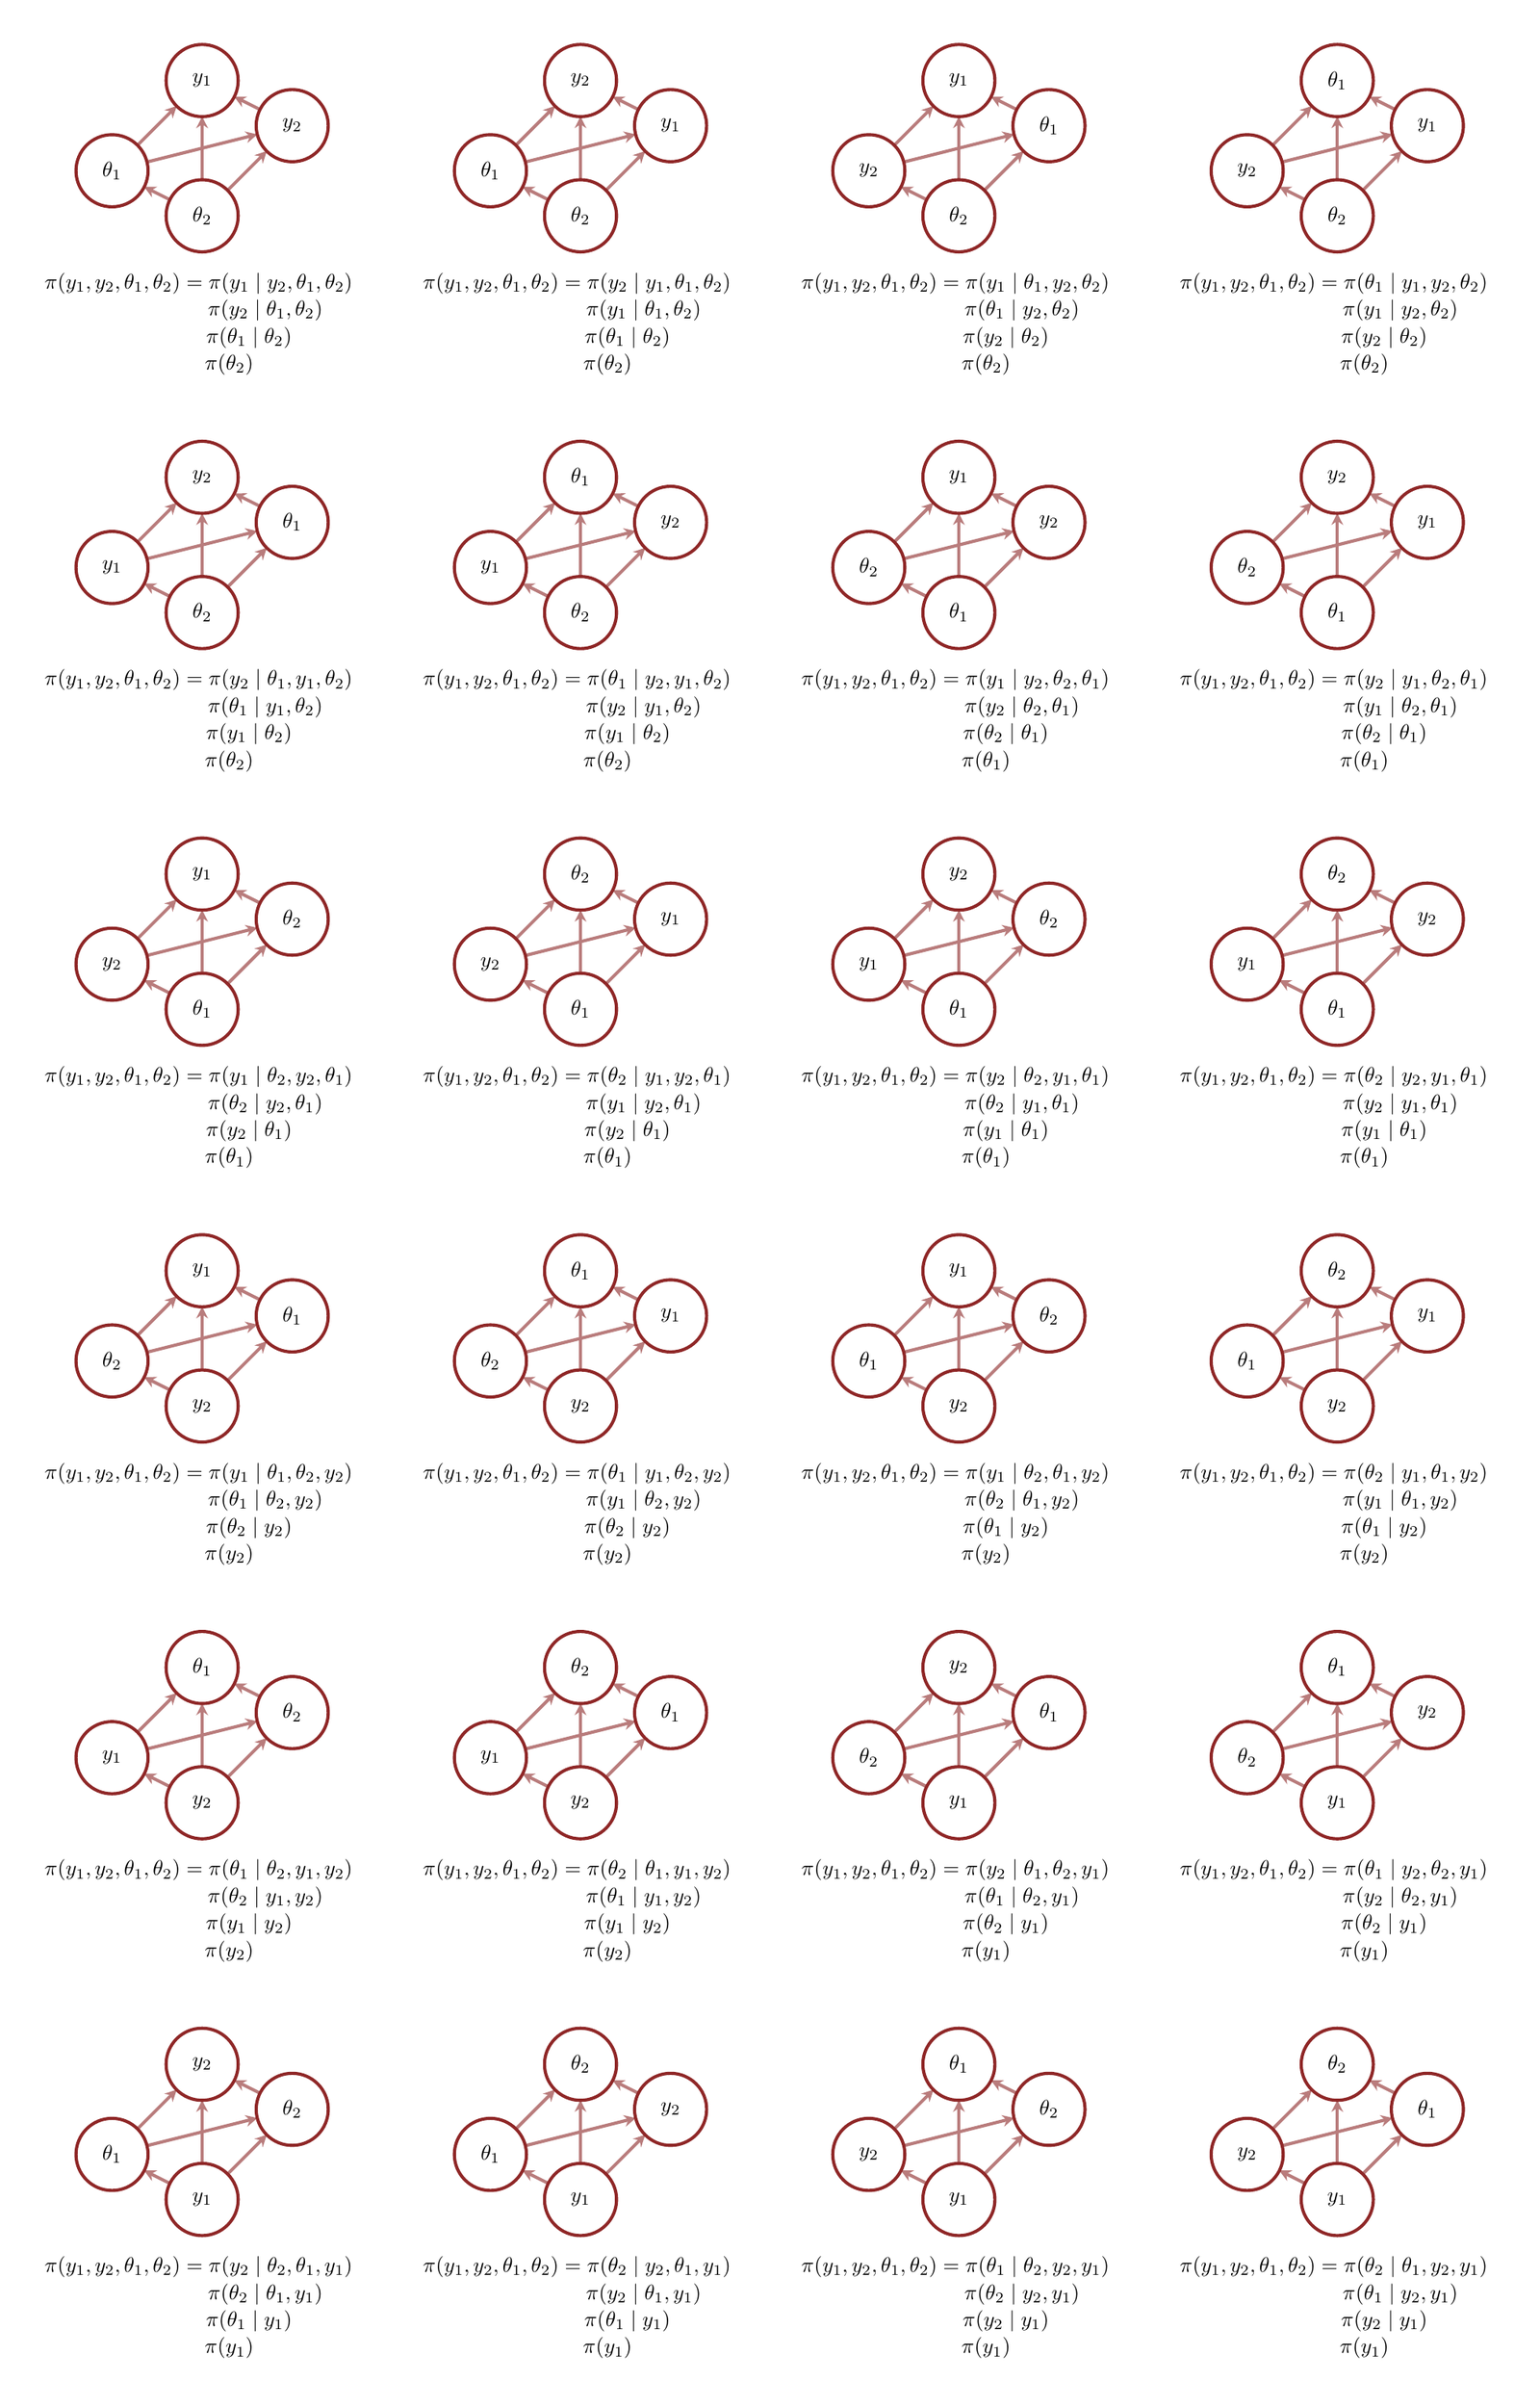
\begin{tikzpicture}[scale=0.3, thick]

\pgfmathsetmacro{\r}{2}

\def\labels{{"y_{1}", "y_{2}", "\theta_{1}", "\theta_{2}"}}
\def\nodexs{{-3, +3, -3, +3}}
\def\nodeys{{+3, +3, -3, -3}}

%\foreach \t/\u/\v/\w [count=\n] in {\a/\b/\c/\d, \a/\b/\d/\c, \b/\c/\d/\a} {

\foreach \t/\u/\v/\w [count=\n] in {3/2/1/0, 3/2/0/1, 3/1/2/0, 3/1/0/2, 3/0/2/1, 3/0/1/2, 
                                    2/3/1/0, 2/3/0/1, 2/1/3/0, 2/1/0/3, 2/0/3/1, 2/0/1/3, 
                                    1/3/2/0, 1/3/0/2, 1/2/3/0, 1/2/0/3, 1/0/3/2, 1/0/2/3, 
                                    0/3/2/1, 0/3/1/2, 0/2/3/1, 0/2/1/3, 0/1/3/2, 0/1/2/3} {

  \pgfmathsetmacro{\dx}{21 * mod(\n - 1, 4)}
  \pgfmathsetmacro{\dy}{-22 * floor((\n - 1) / 4)}

  \pgfmathsetmacro{\Al}{\labels[\t]}
  \pgfmathsetmacro{\Bl}{\labels[\u]}
  \pgfmathsetmacro{\Cl}{\labels[\v]}
  \pgfmathsetmacro{\Dl}{\labels[\w]}
  
  \pgfmathsetmacro{\Ax}{\nodexs[\t]}
  \pgfmathsetmacro{\Ay}{\nodeys[\t]}

  \pgfmathsetmacro{\Bx}{\nodexs[\u]}
  \pgfmathsetmacro{\By}{\nodeys[\u]}
  
  \pgfmathsetmacro{\Cx}{\nodexs[\v]}
  \pgfmathsetmacro{\Cy}{\nodeys[\v]}
  
  \pgfmathsetmacro{\Dx}{\nodexs[\w]}
  \pgfmathsetmacro{\Dy}{\nodeys[\w]}
  
  \begin{scope}[shift={(\dx, \dy)}]
    \draw[white] (-10, -14) rectangle (10, 7);
    
    %\draw[-{Stealth[length=5.5pt, width=5.5pt]}, shorten >=17, color=mid, line width=1.5] (\Ax, \Ay) -- (\Bx, \By);
    %\draw[-{Stealth[length=5.5pt, width=5.5pt]}, shorten >=17, color=mid, line width=1.5] (\Ax, \Ay) -- (\Cx, \Cy);
    %\draw[-{Stealth[length=5.5pt, width=5.5pt]}, shorten >=17, color=mid, line width=1.5] (\Ax, \Ay) -- (\Dx, \Dy);
    
    %\draw[-{Stealth[length=5.5pt, width=5.5pt]}, shorten >=17, color=mid, line width=1.5] (\Bx, \By) -- (\Cx, \Cy);
    %\draw[-{Stealth[length=5.5pt, width=5.5pt]}, shorten >=17, color=mid, line width=1.5] (\Bx, \By) -- (\Dx, \Dy);
    
    %\draw[-{Stealth[length=5.5pt, width=5.5pt]}, shorten >=17, color=mid, line width=1.5] (\Cx, \Cy) -- (\Dx, \Dy);
    
    %\filldraw[fill=white, draw=dark, line width=1.5] (-3, +3) circle (\r)
    %node[color=black] { $y_{1}$ };
      
    %\filldraw[fill=white, draw=dark, line width=1.5] (+3, +3) circle (\r)
    %node[color=black] { $y_{2}$ };
      
    %\filldraw[fill=white, draw=dark, line width=1.5] (-3, -3) circle (\r)
    %node[color=black] { $\theta_{1}$ };
    
    %\filldraw[fill=white, draw=dark, line width=1.5] (+3, -3) circle (\r)
    %node[color=black] { $\theta_{2}$ };

    \draw[-{Stealth[length=5.5pt, width=5.5pt]}, shorten >=17, color=mid, line width=1.5] (+0, -3.75) -- (-5, -1.25);
    \draw[-{Stealth[length=5.5pt, width=5.5pt]}, shorten >=17, color=mid, line width=1.5] (+0, -3.75) -- (+5, +1.25);
    \draw[-{Stealth[length=5.5pt, width=5.5pt]}, shorten >=17, color=mid, line width=1.5] (+0, -3.75) -- (+0, +3.75);
    
    \draw[-{Stealth[length=5.5pt, width=5.5pt]}, shorten >=17, color=mid, line width=1.5] (-5, -1.25) -- (+5, +1.25);
    \draw[-{Stealth[length=5.5pt, width=5.5pt]}, shorten >=17, color=mid, line width=1.5] (-5, -1.25) -- (+0, +3.75);
    
    \draw[-{Stealth[length=5.5pt, width=5.5pt]}, shorten >=17, color=mid, line width=1.5] (+5, +1.25) -- (+0, +3.75);
    
    \filldraw[fill=white, draw=dark, line width=1.5] (0, 3.75) circle (\r)
    node[color=black] { $\Dl$ };
      
    \filldraw[fill=white, draw=dark, line width=1.5] (+5, 1.25) circle (\r)
    node[color=black] { $\Cl$ };
      
    \filldraw[fill=white, draw=dark, line width=1.5] (-5, -1.25) circle (\r)
    node[color=black] { $\Bl$ };
    
    \filldraw[fill=white, draw=dark, line width=1.5] (0, -3.75) circle (\r)
    node[color=black] { $\Al$ };
    
    \node[align=center] at (0, -7.5) { $\pi(y_{1}, y_{2}, \theta_{1}, \theta_{2}) = \pi(\Dl \mid \Cl, \Bl, \Al)$ };
    \node[align=center] at (3.7, -9) { $\pi(\Cl \mid \Bl, \Al)$ };
    \node[align=center] at (2.8, -10.5) { $\pi(\Bl \mid \Al)$ };
    \node[align=center] at (1.7, -12) { $\pi(\Al)$ };
    
  \end{scope}
}

\end{tikzpicture}

\end{document}  